\documentclass[10pt]{article}

% Lines beginning with the percent sign are comments
% This file has been commented to help you understand more about LaTeX

% DO NOT EDIT THE LINES BETWEEN THE TWO LONG HORIZONTAL LINES

%---------------------------------------------------------------------------------------------------------

% Packages add extra functionality.
\usepackage{times,graphicx,epstopdf,fancyhdr,amsfonts,amsthm,amsmath,algorithm,algorithmic,xspace,hyperref}
\usepackage[left=1in,top=1in,right=1in,bottom=1in]{geometry}
\usepackage{sect sty}	%For centering section headings
\usepackage{enumerate}	%Allows more labeling options for enumerate environments 
\usepackage{epsfig}
\usepackage[space]{grffile}
\usepackage{booktabs}

% This will set LaTeX to look for figures in the same directory as the .tex file
\graphicspath{.} % The dot means current directory.

\pagestyle{fancy}

\lhead{\YOURID}
\chead{Midterm: \RRNumber}
\rhead{\today}
\lfoot{CSCI 334: Principles of Programming Languages}
\cfoot{\thepage}
\rfoot{Fall 2018}

% Some commands for changing header and footer format
\renewcommand{\headrulewidth}{0.4pt}
\renewcommand{\headwidth}{\textwidth}
\renewcommand{\footrulewidth}{0.4pt}

% These let you use common environments
\newtheorem{claim}{Claim}
\newtheorem{definition}{Definition}
\newtheorem{theorem}{Theorem}
\newtheorem{lemma}{Lemma}
\newtheorem{observation}{Observation}
\newtheorem{question}{Question}

\setlength{\parindent}{0cm}


%---------------------------------------------------------------------------------------------------------

% DON'T CHANGE ANYTHING ABOVE HERE

% Edit below as instructed
\newcommand{\YOURID}{Noah Cowit}	% Replace 3023867 with your ID for the course
\newcommand{\RRNumber}{Test Corrections}	% Replace 0 with the actual problem set #
\newcommand{\ProblemHeader}	% Don't change this!

\begin{document}

\vspace{\baselineskip}	% Add some vertical space

\begin{enumerate}

\item
  \textbf{q1h}

  My answer: true

  \vspace{\baselineskip}
  
  New answer: false

  \vspace{\baselineskip}

 Explaination:  A literal value is evaluated as it's declaration. A String literal `time` is evaluated as `time` and an int literal 1 is evaluated as 1. Thus the program has access to the values of literal types. They are allocated statically by the compiler and usually stored in read only memory. They do not need to be allocated.

  
 \item
  \textbf{q1j}

  My answer: true

  \vspace{\baselineskip}
  
  New answer: false

  \vspace{\baselineskip}

  Arguments are not passed by pointer in C. They are passed by value. This is relatively standard for programing langauges.

 \item
   \textbf{q2}
   
   My original answer: I thought that there was a problem with memory allocation, but I had a very wrong idea about where this memory allocation problem happened, I was debating if the issue was with a double free at the end, or a problem with using arrarr that wasn't the real issue. Either way, I was wrong. I thought that this line:

   \begin{verbatim}
     char **arrarr = malloc(sizeof(char*) *n)
   \end{verbatim}

   was enough to allocate an array of C-Strings. Now I understand that this line only allocates memory for the pointers to C-Strings.

   \vspace{\baselineskip}

   \vspace{\baselineskip}

   New answer: The first attempt to write to arrarr is inside of the randomString function, by memset:

      \begin{verbatim}
        memset(arr, '\0', len+1);
      \end{verbatim}

      Before this function is called, the call stack looks as follows:

 \begin{center}
    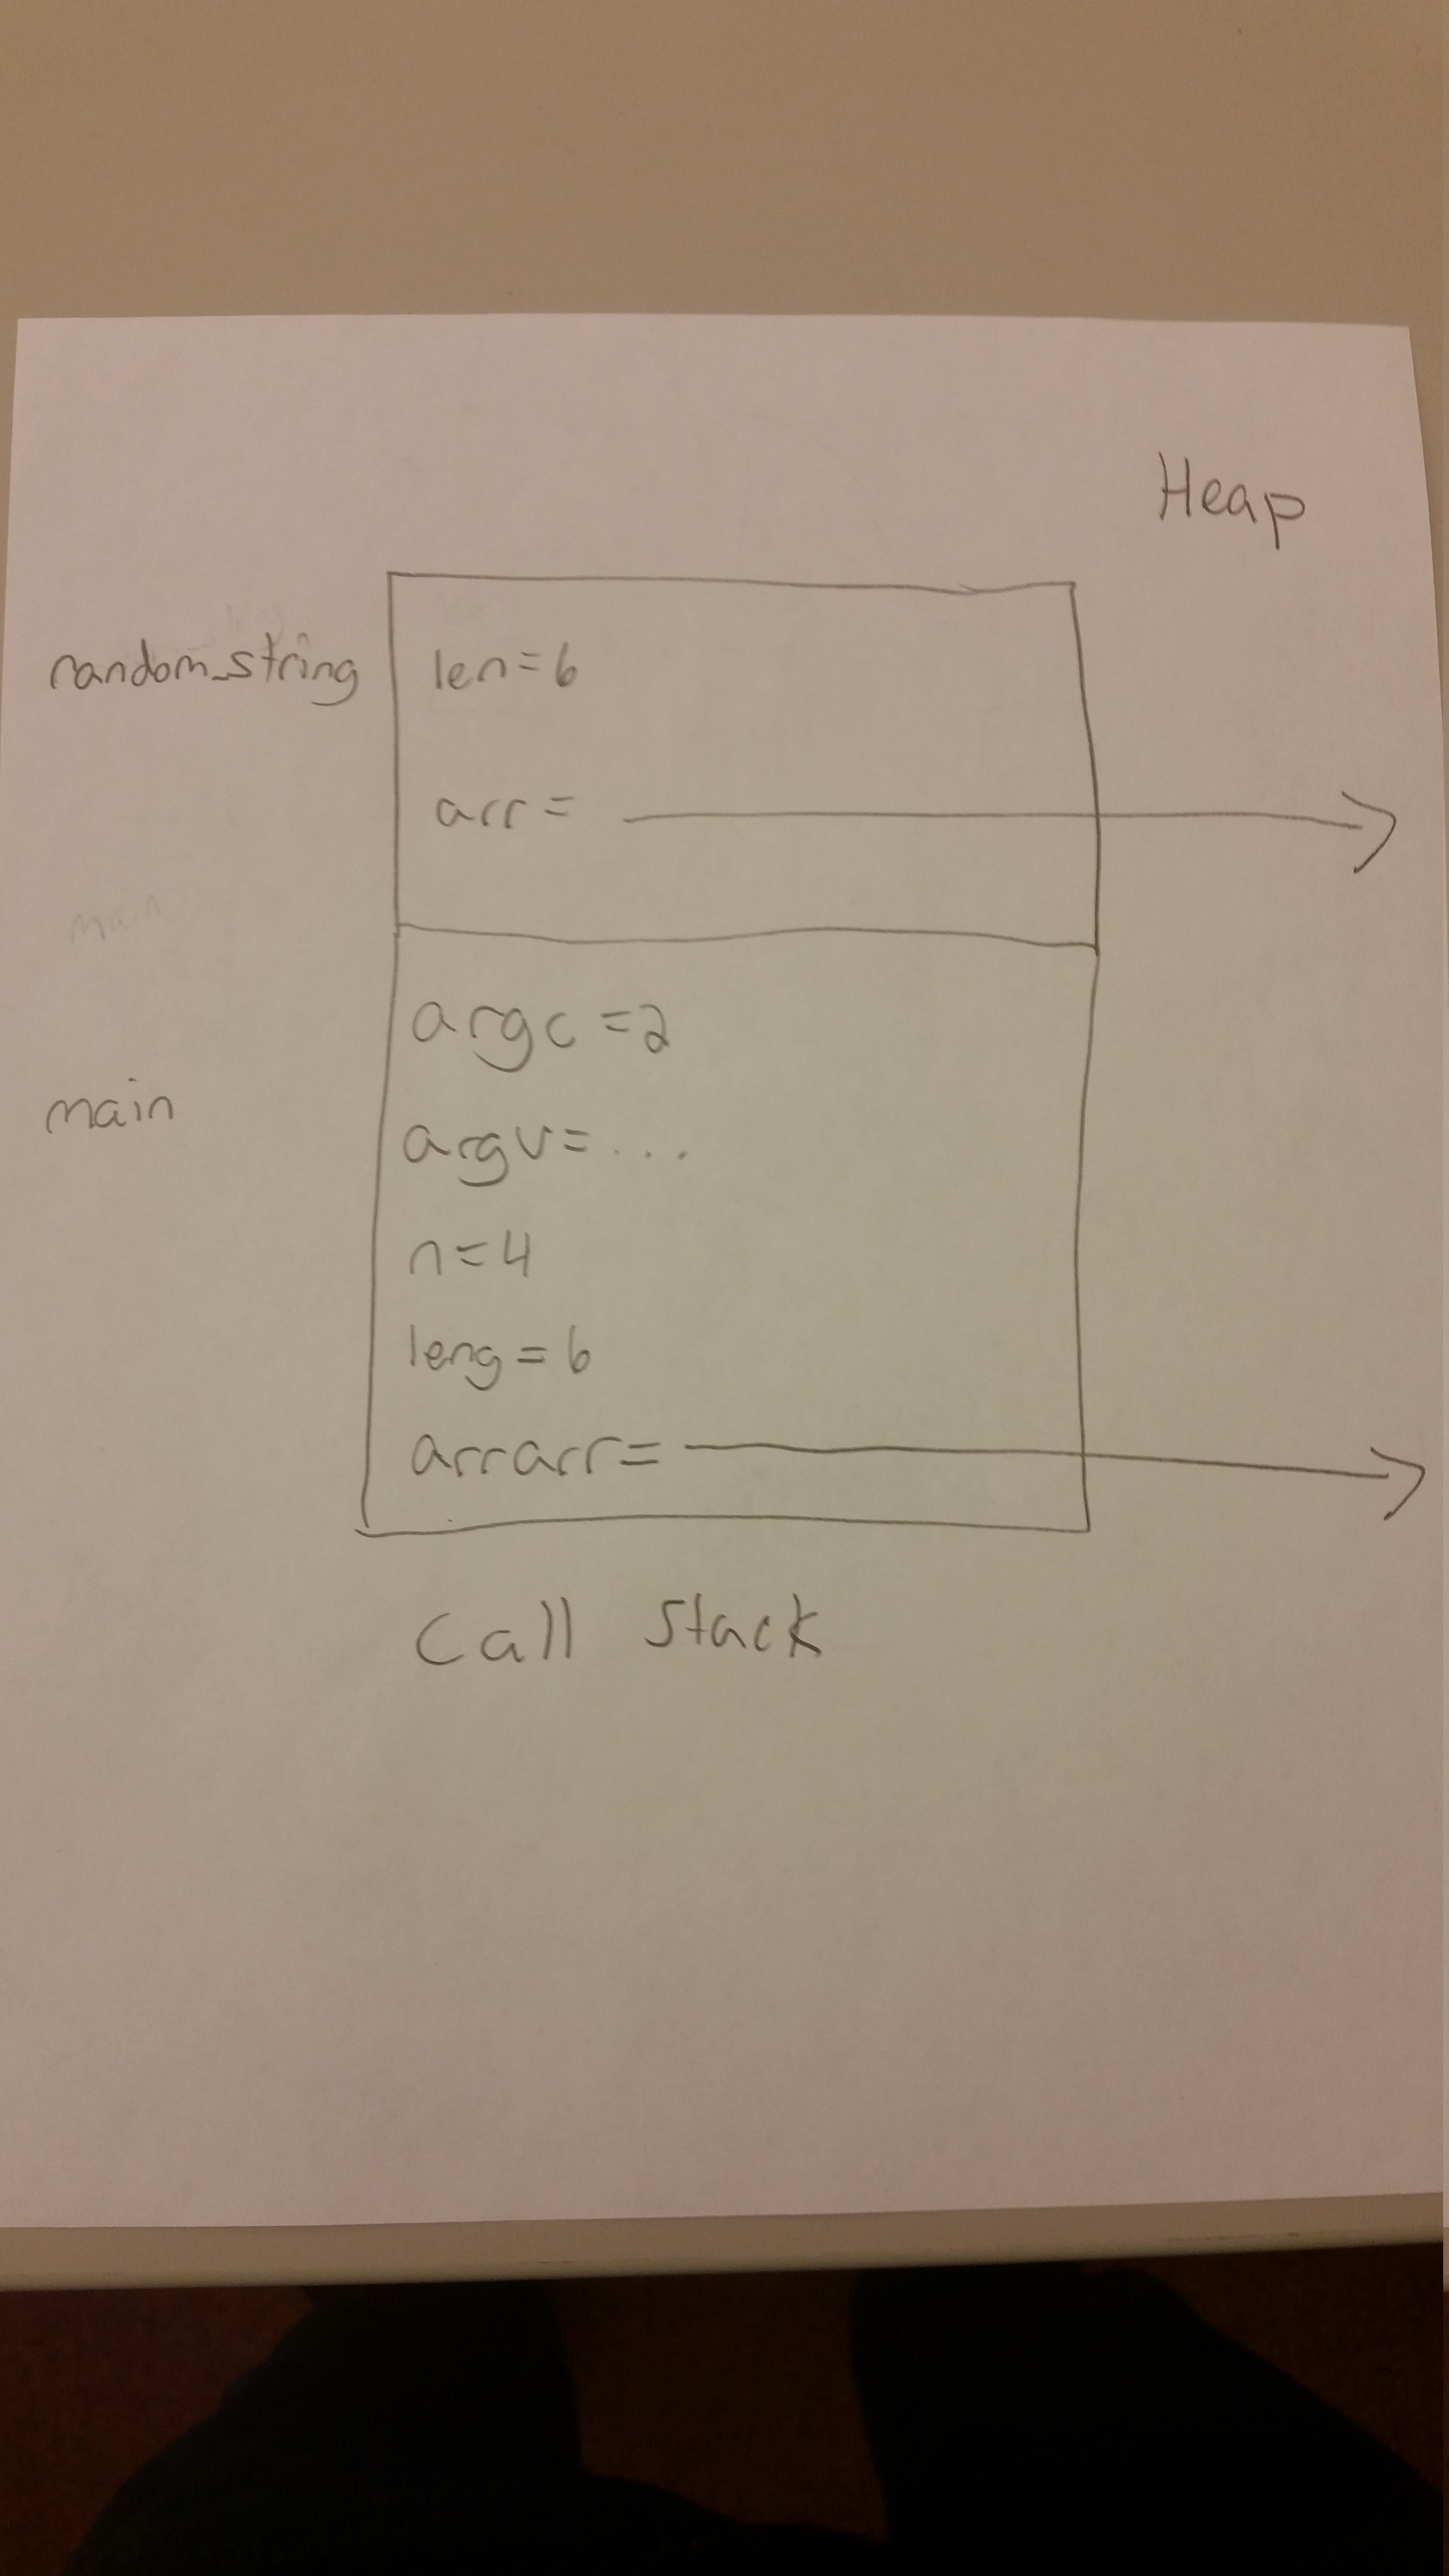
\includegraphics[width=0.33\textwidth]{images/ccc1.jpg}
 \end{center}

 arrarr has been alocated and with it, the memory for C-string pointers on the heap. Visually, this can be displayed like this:
  
 \begin{center}
    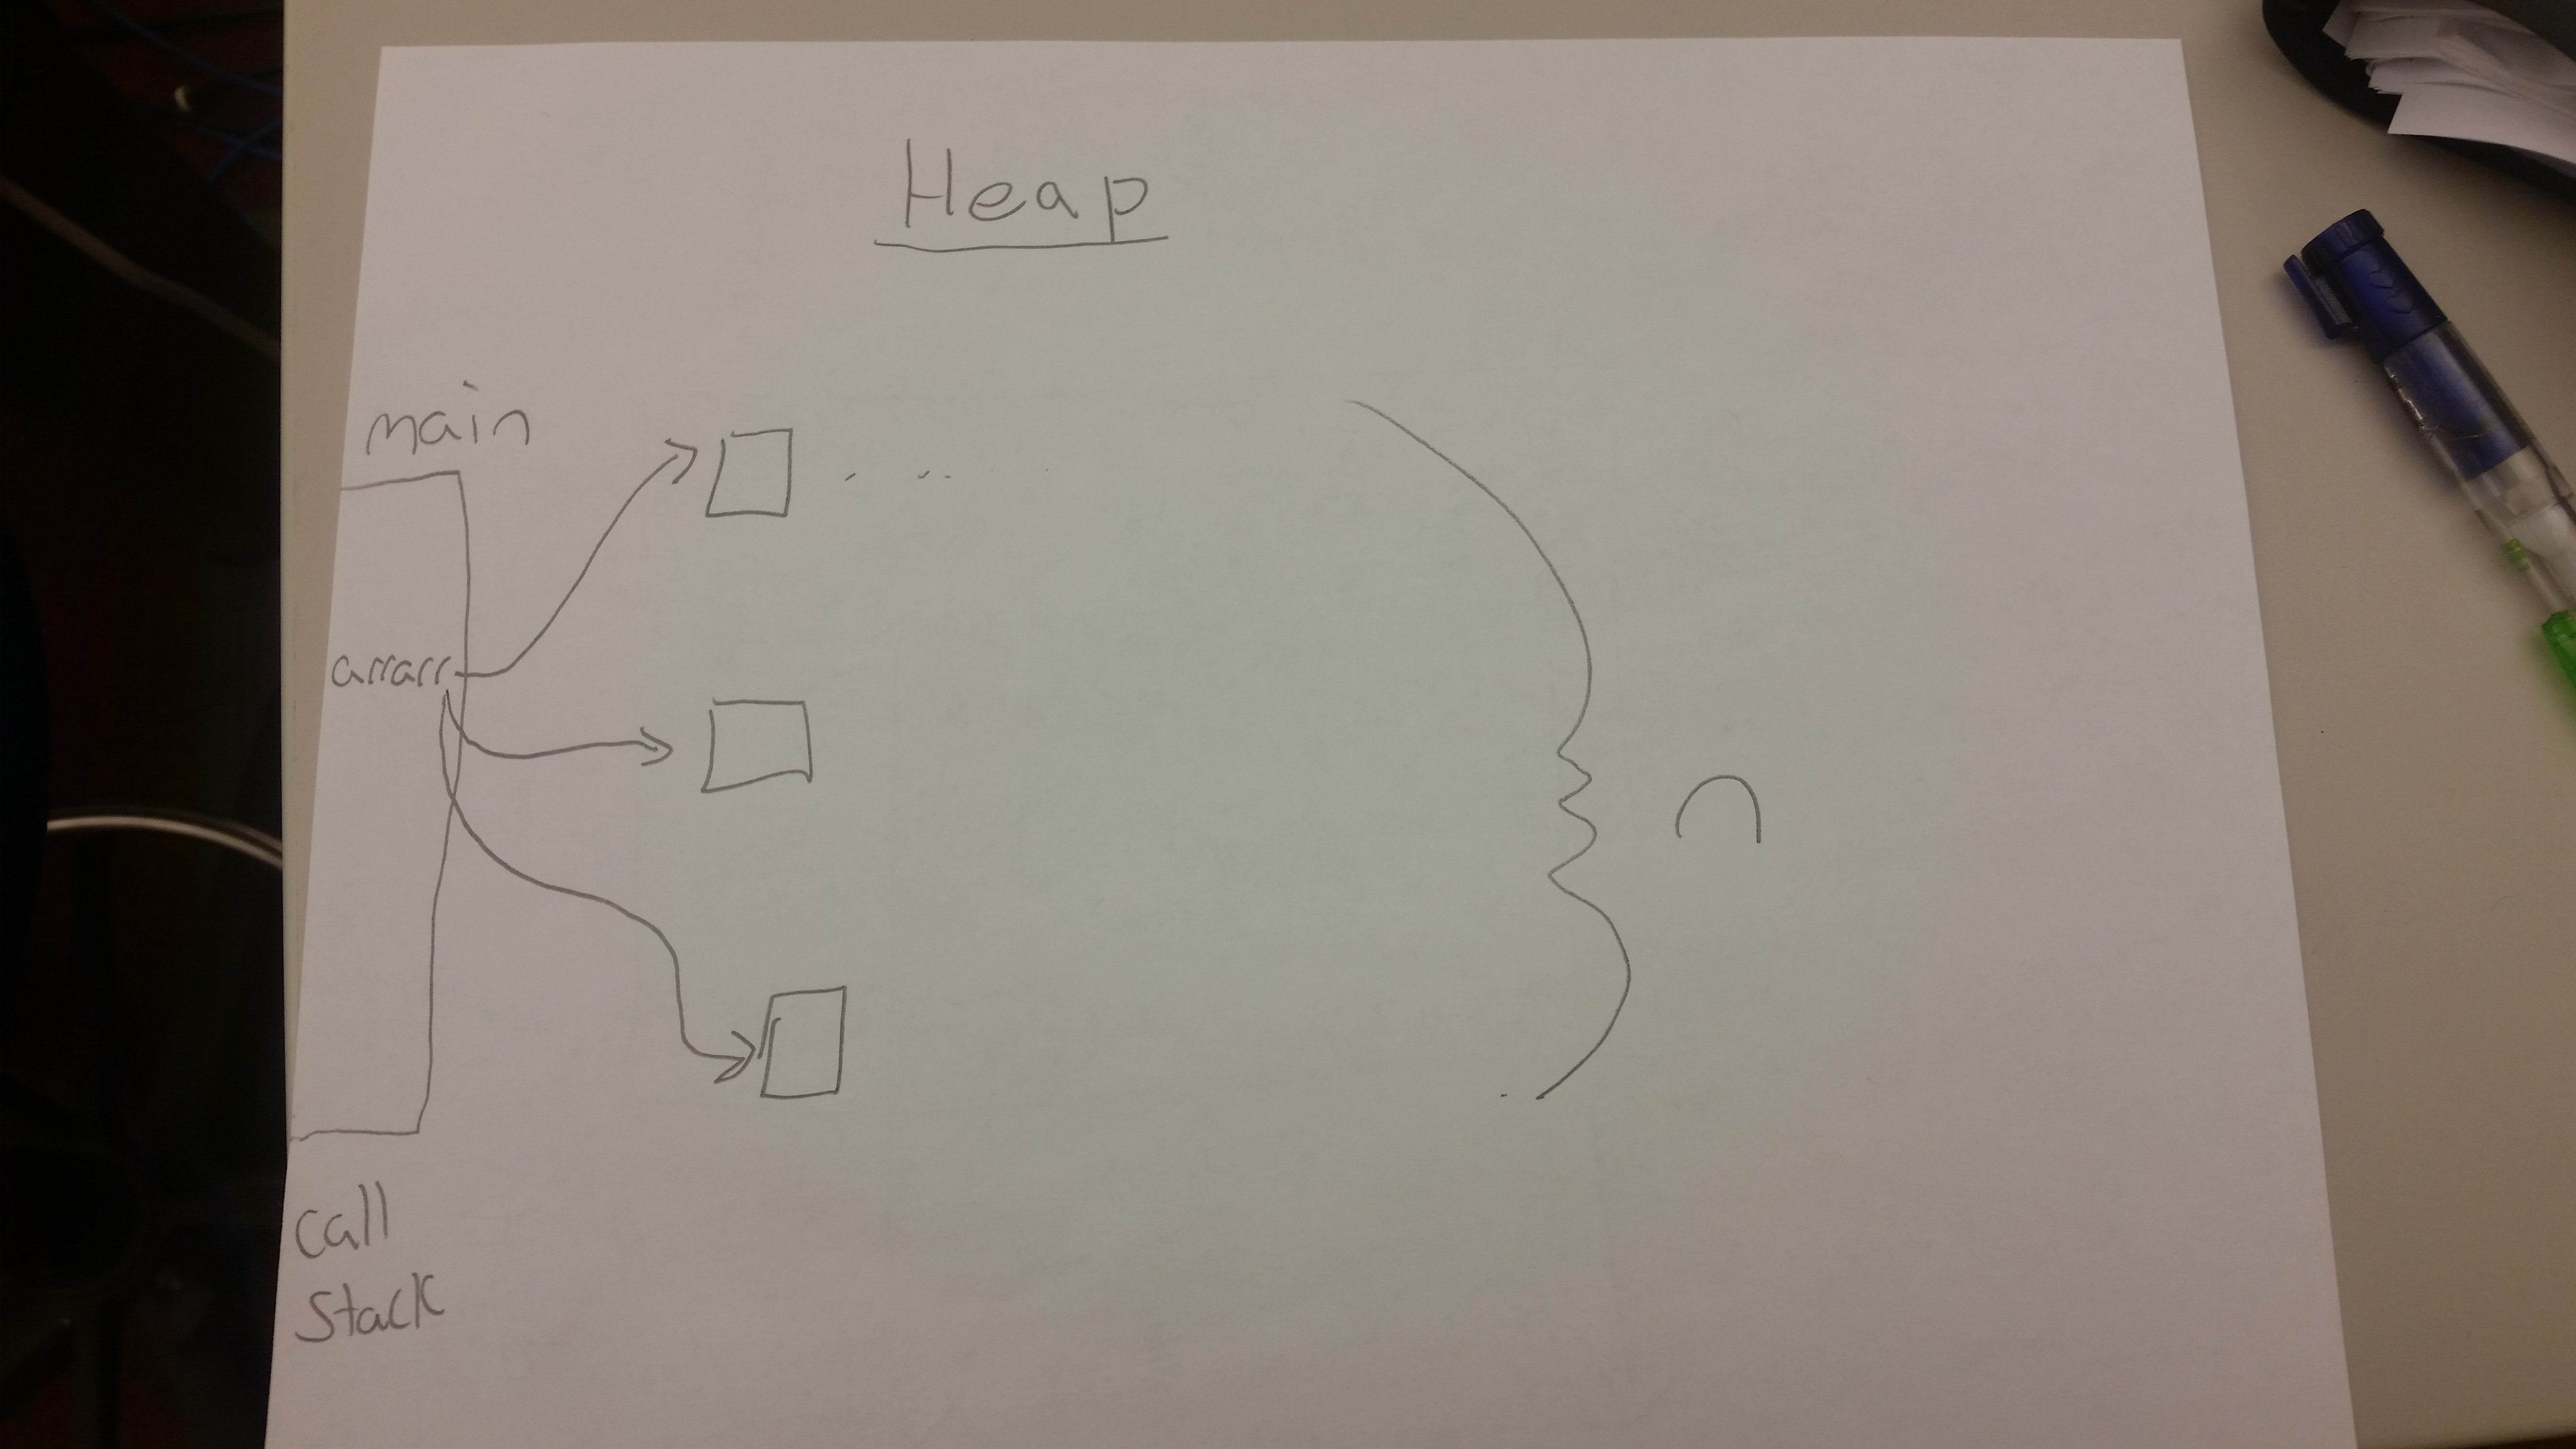
\includegraphics[width=0.33\textwidth]{images/c2.jpg}
 \end{center}

As we can see the pointers have been allocated, yet the memory for the values of the strings (the set of chars in the C-string) has not been allocated yet. This leads to the following behavior when randomstring is called:
 
  \begin{center}
    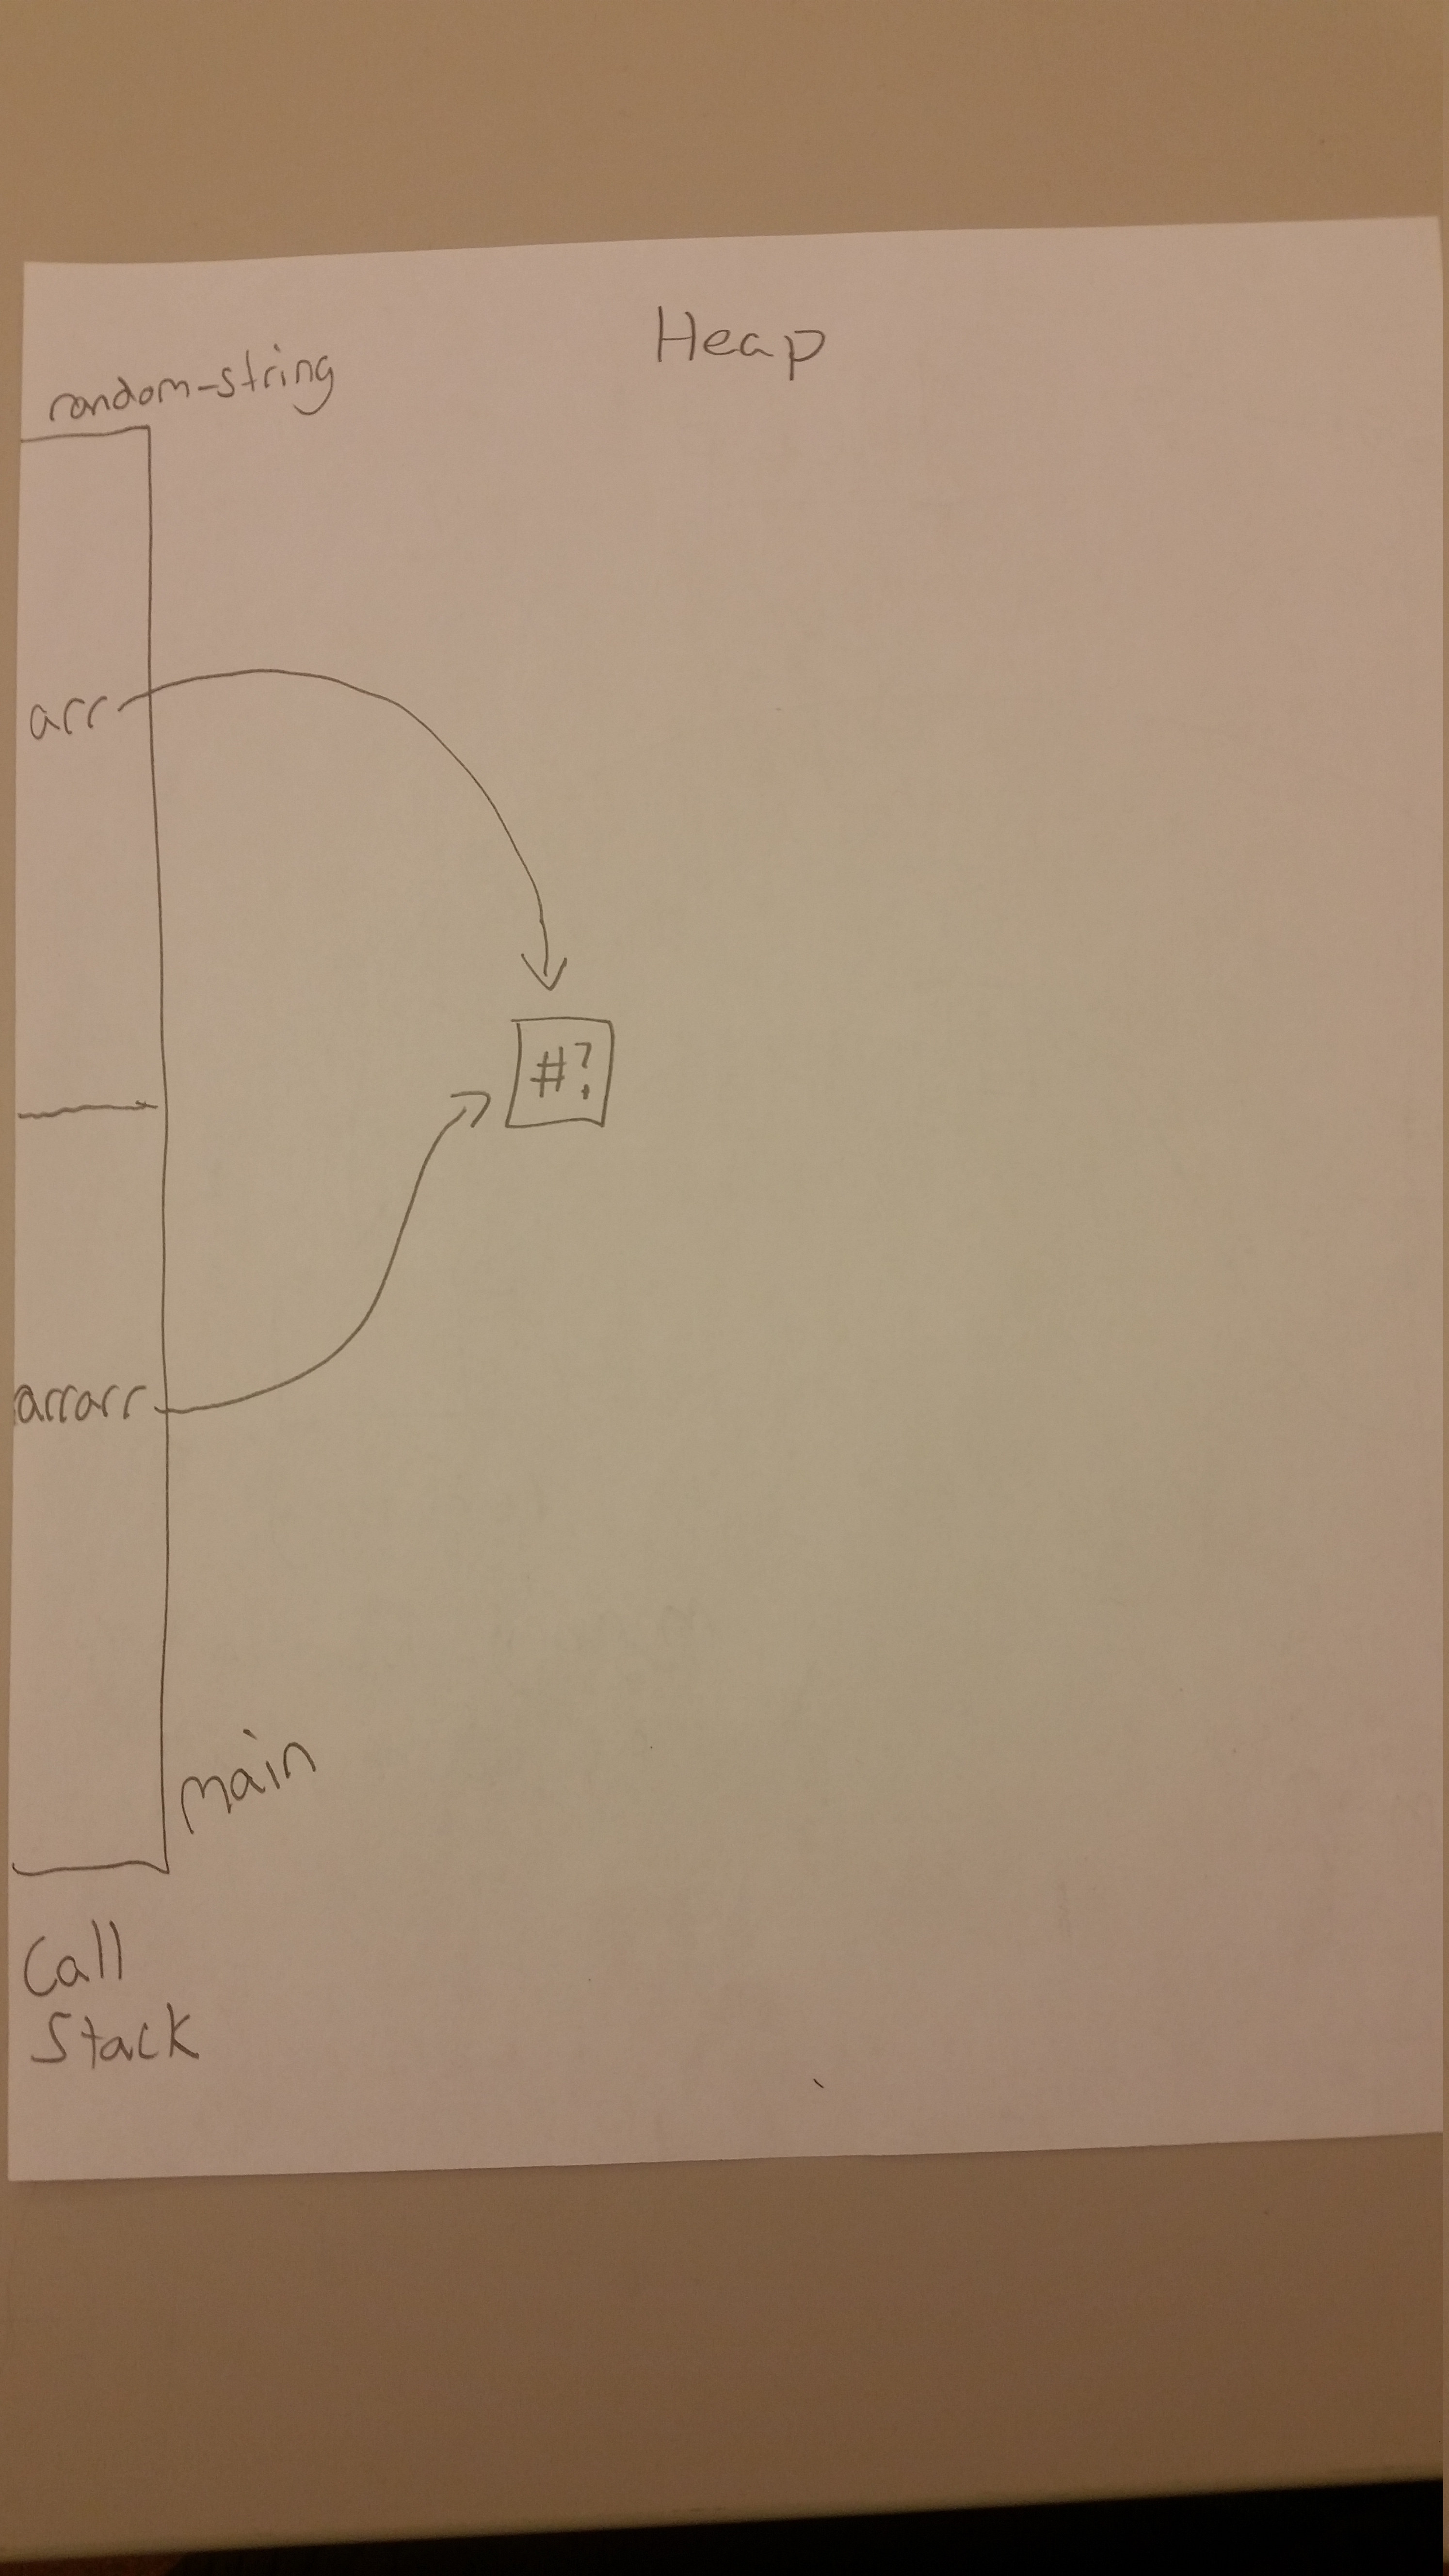
\includegraphics[width=0.33\textwidth]{images/c3.jpg}
  \end{center}

  Frist we see arr(passed to randomString as a pointer to arrarr) try to write to the memory pointed to by arrarr. But all it processes is a pointer. Memory for the values of arrarr have not been allocated. If a value is stored at the location pointed to, it is interpreted as another pointer, leading to the situation below:

   \begin{center}
    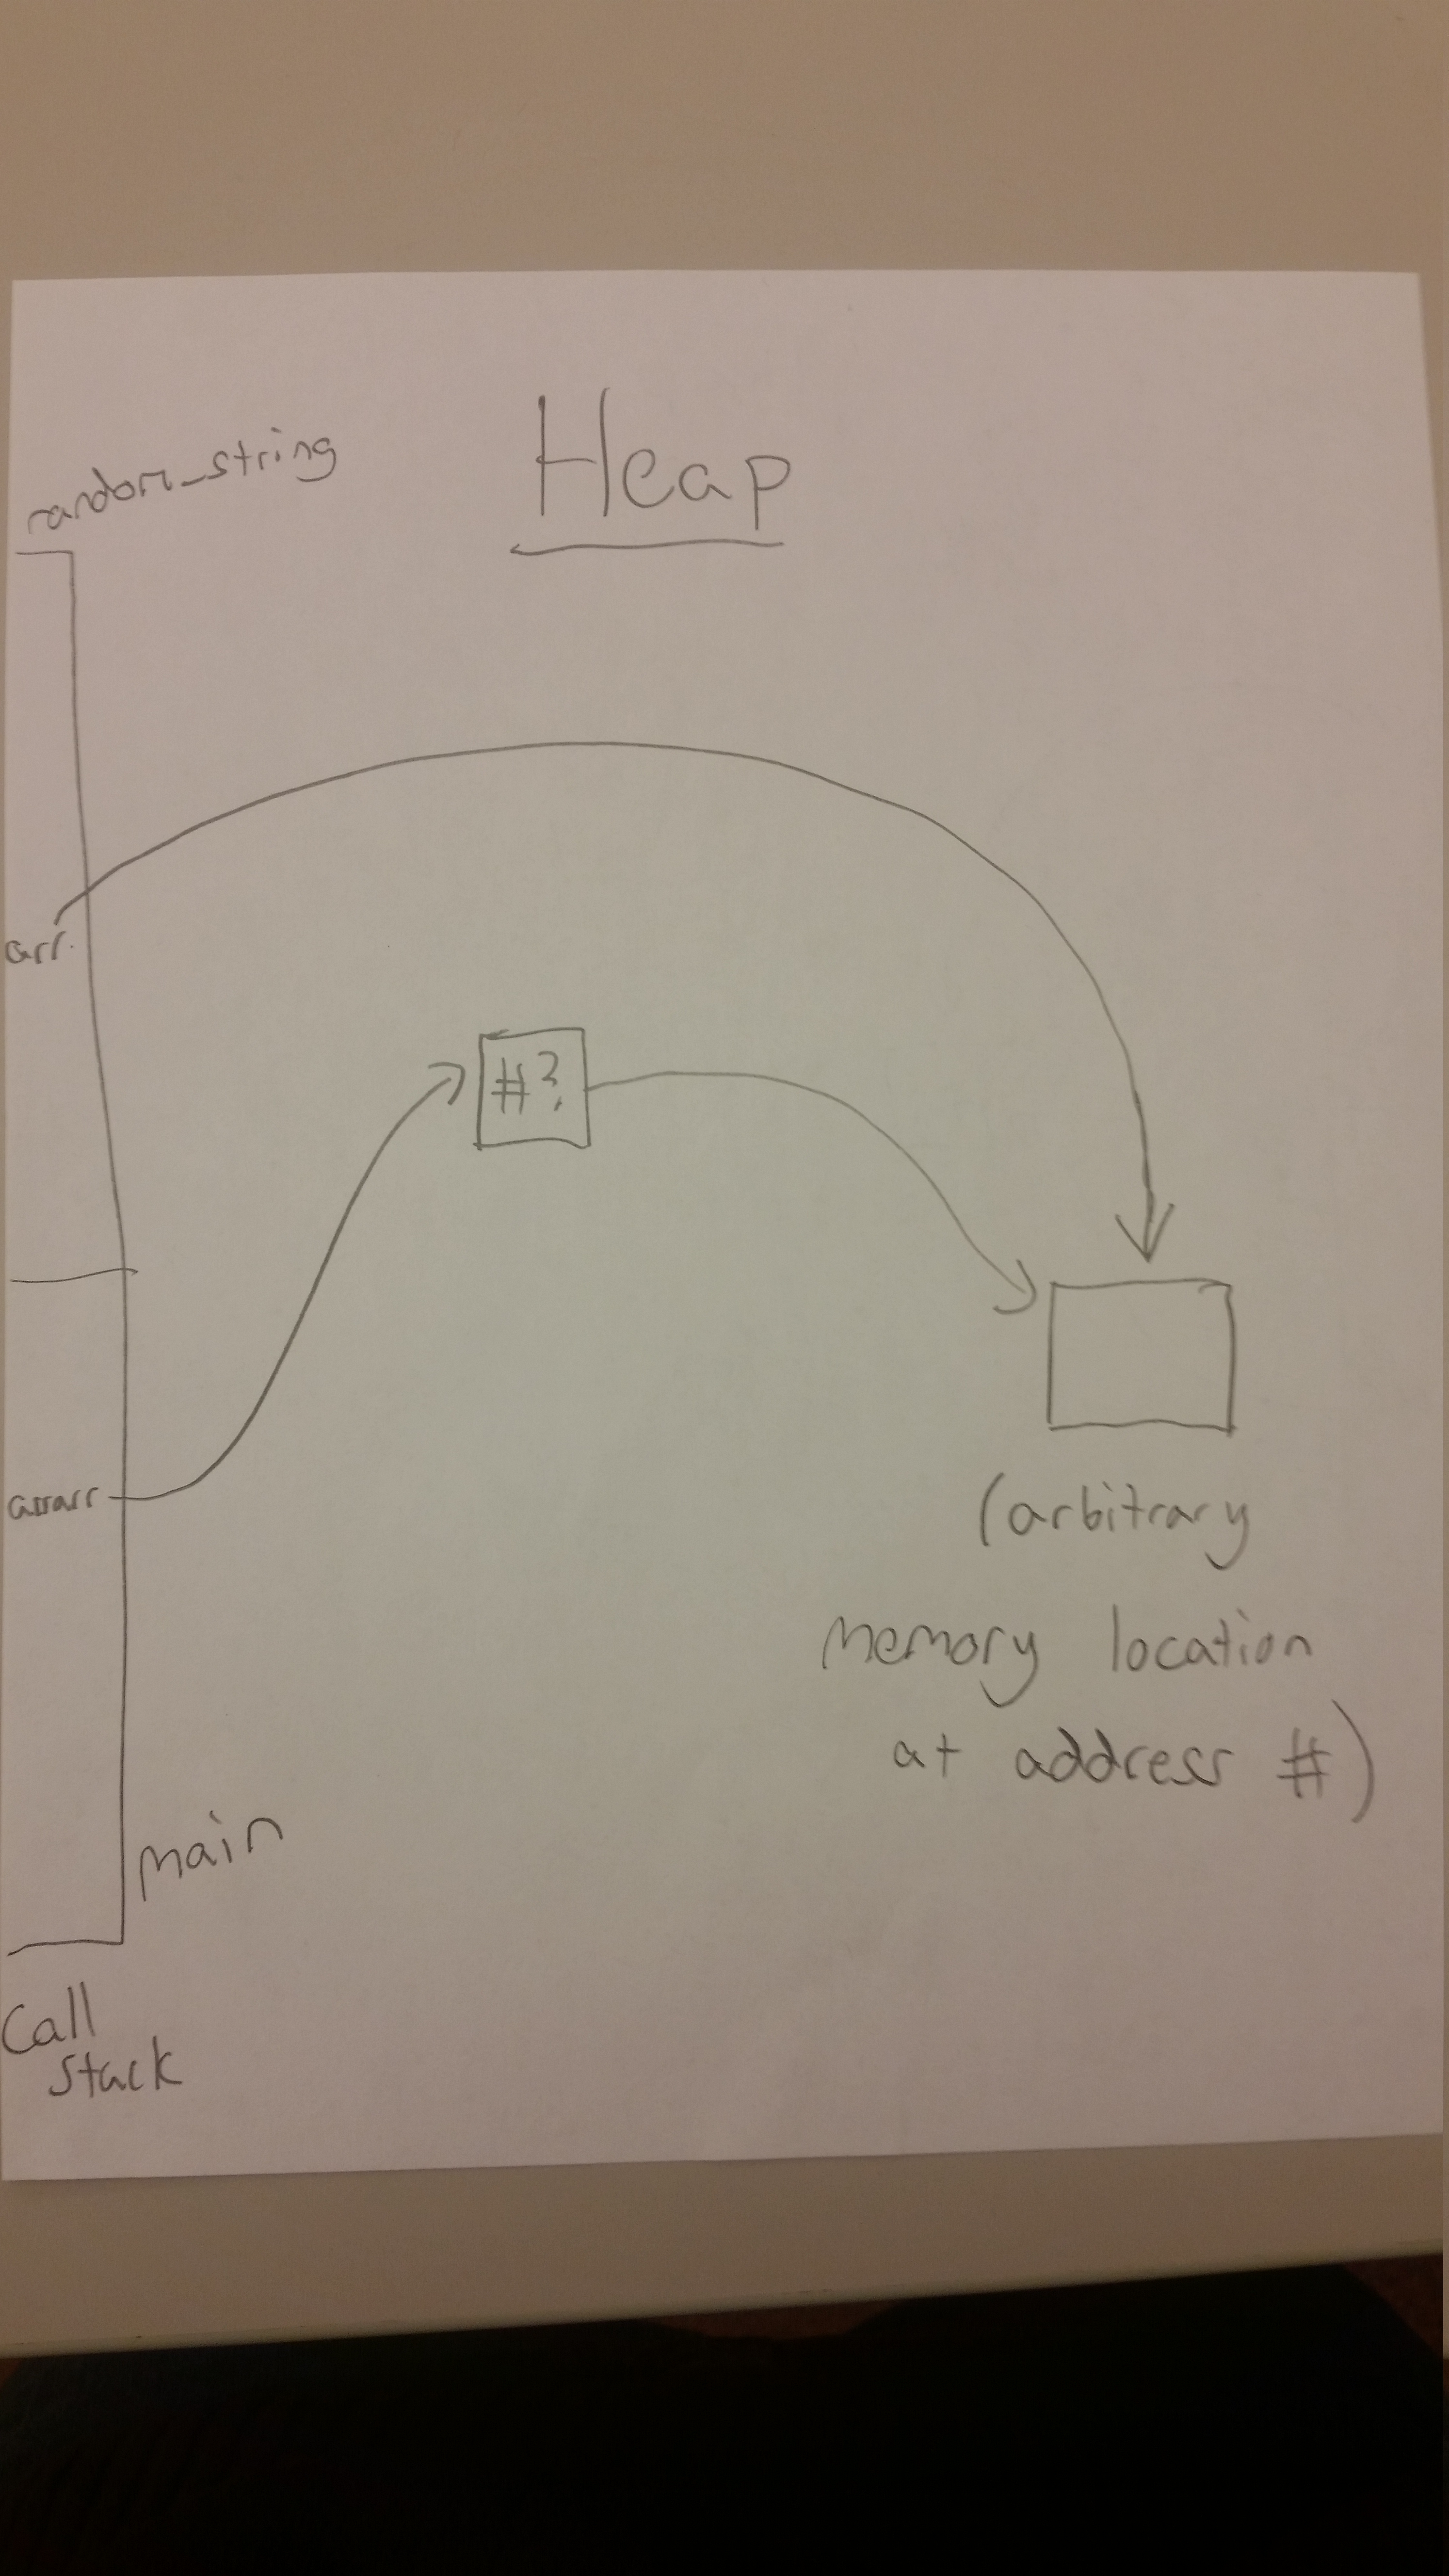
\includegraphics[width=0.33\textwidth]{images/ccc4.jpg}
   \end{center}

   randomString(and memset in particular) tries to write to an arbitrary memory location, at the address of the value pointed to by arrarr. If this is memory which is not allowed to be overwritten, a segmentation fault occurs and the program crashes.

 \vspace{\baselineskip}
   
   Hence the patch is in the for loop which calls the randomstring function. It is placed directly before the function is called:

        \begin{verbatim}
          arrarr[i] =malloc(sizeof(char) *(len+1));
          mcheck(arrarr[i]);
          
          randomString(arrarr[i]);
        \end{verbatim}

        The first line of the patch allocates memory for the char values of 1 C-string of length len (it is written as len+1 to allow space for the terminating null terminator in the C-string). These values will be written to by the randomString call. Then the for loop will iterate or terminate based on the condition (i<n). The program will continue to allocate memory for C-strings, and write to C-strings with randomString, until this point. The final line of the patch is a basic check to see if the memory allocation succeeded.

  \vspace{\baselineskip}


  
 \item
  \textbf{q3a}

  my answer: The sentance is valid. (photo attached)

     \begin{center}
    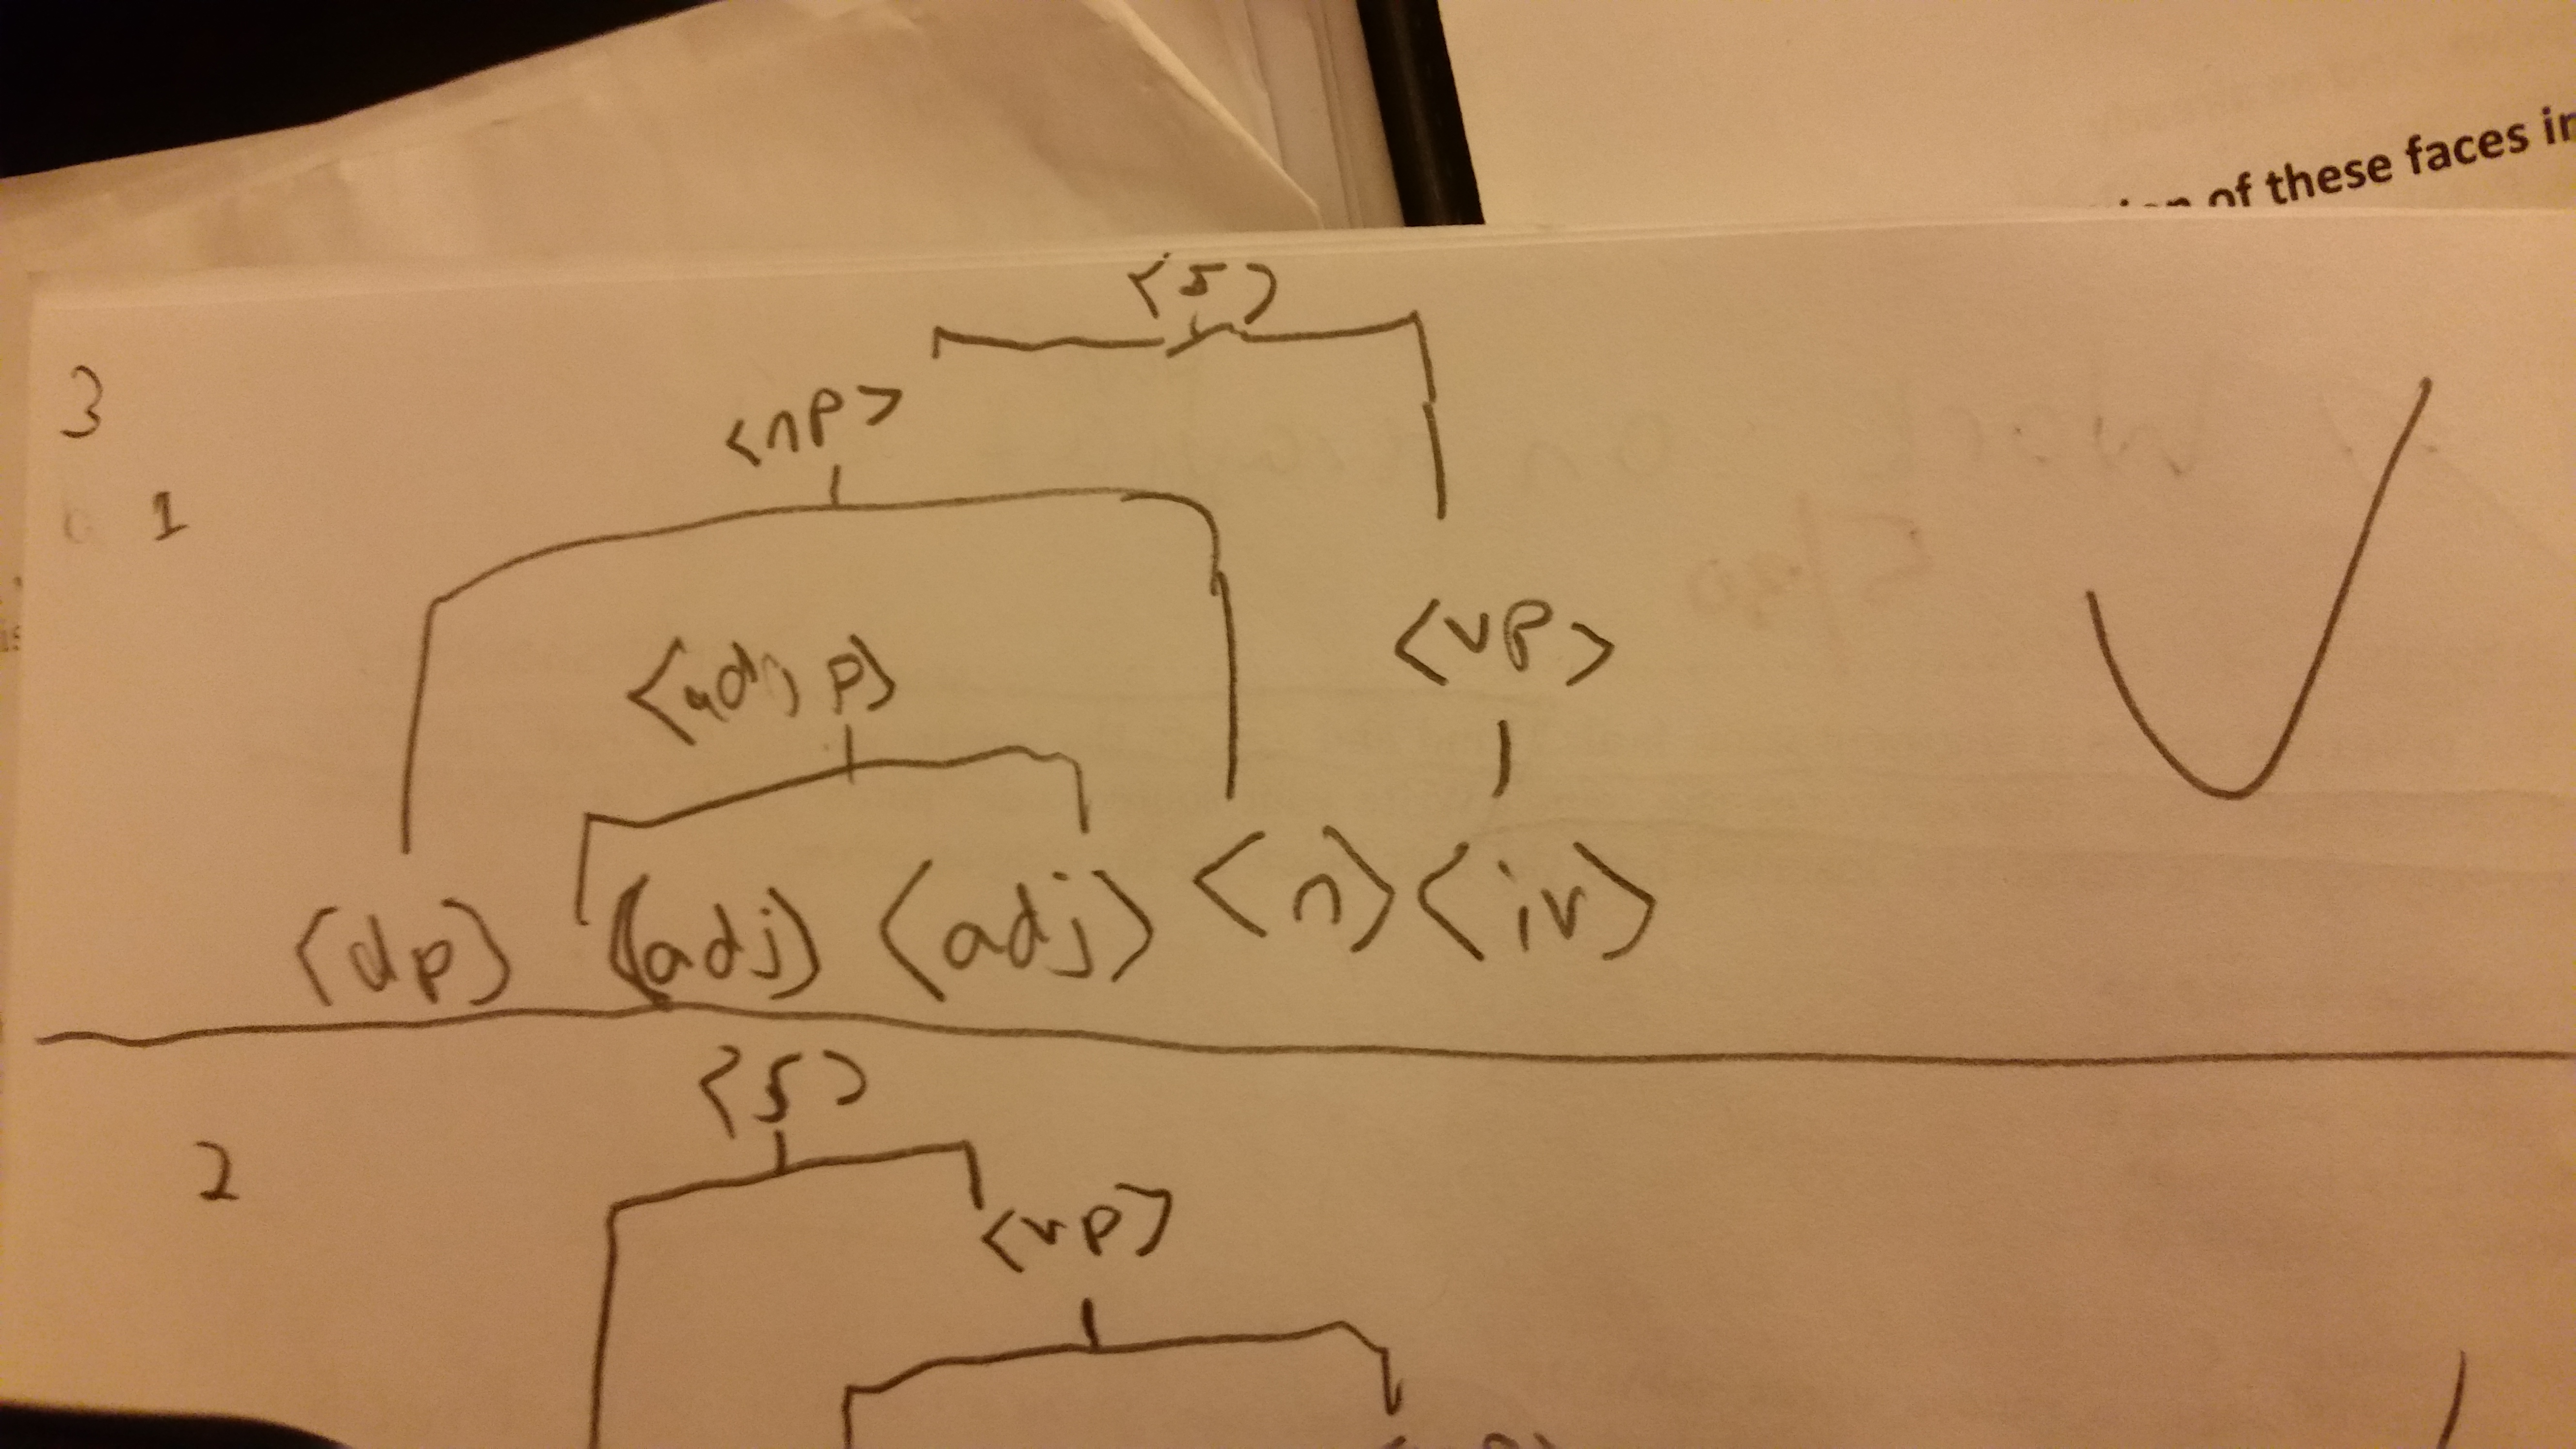
\includegraphics[width=0.33\textwidth]{images/m1.jpg}
  \end{center}

  new answer: The sentance is invalid.

  \vspace{\baselineskip}

  Explaination: The word `The` is not present in the grammar for the language. It should have been `the`. Then the parse tree created would work out. I did not realize that the T was capitalized.
 

 \item
  \textbf{q4}

  my answer: inf (photo attached)

    \begin{center}
    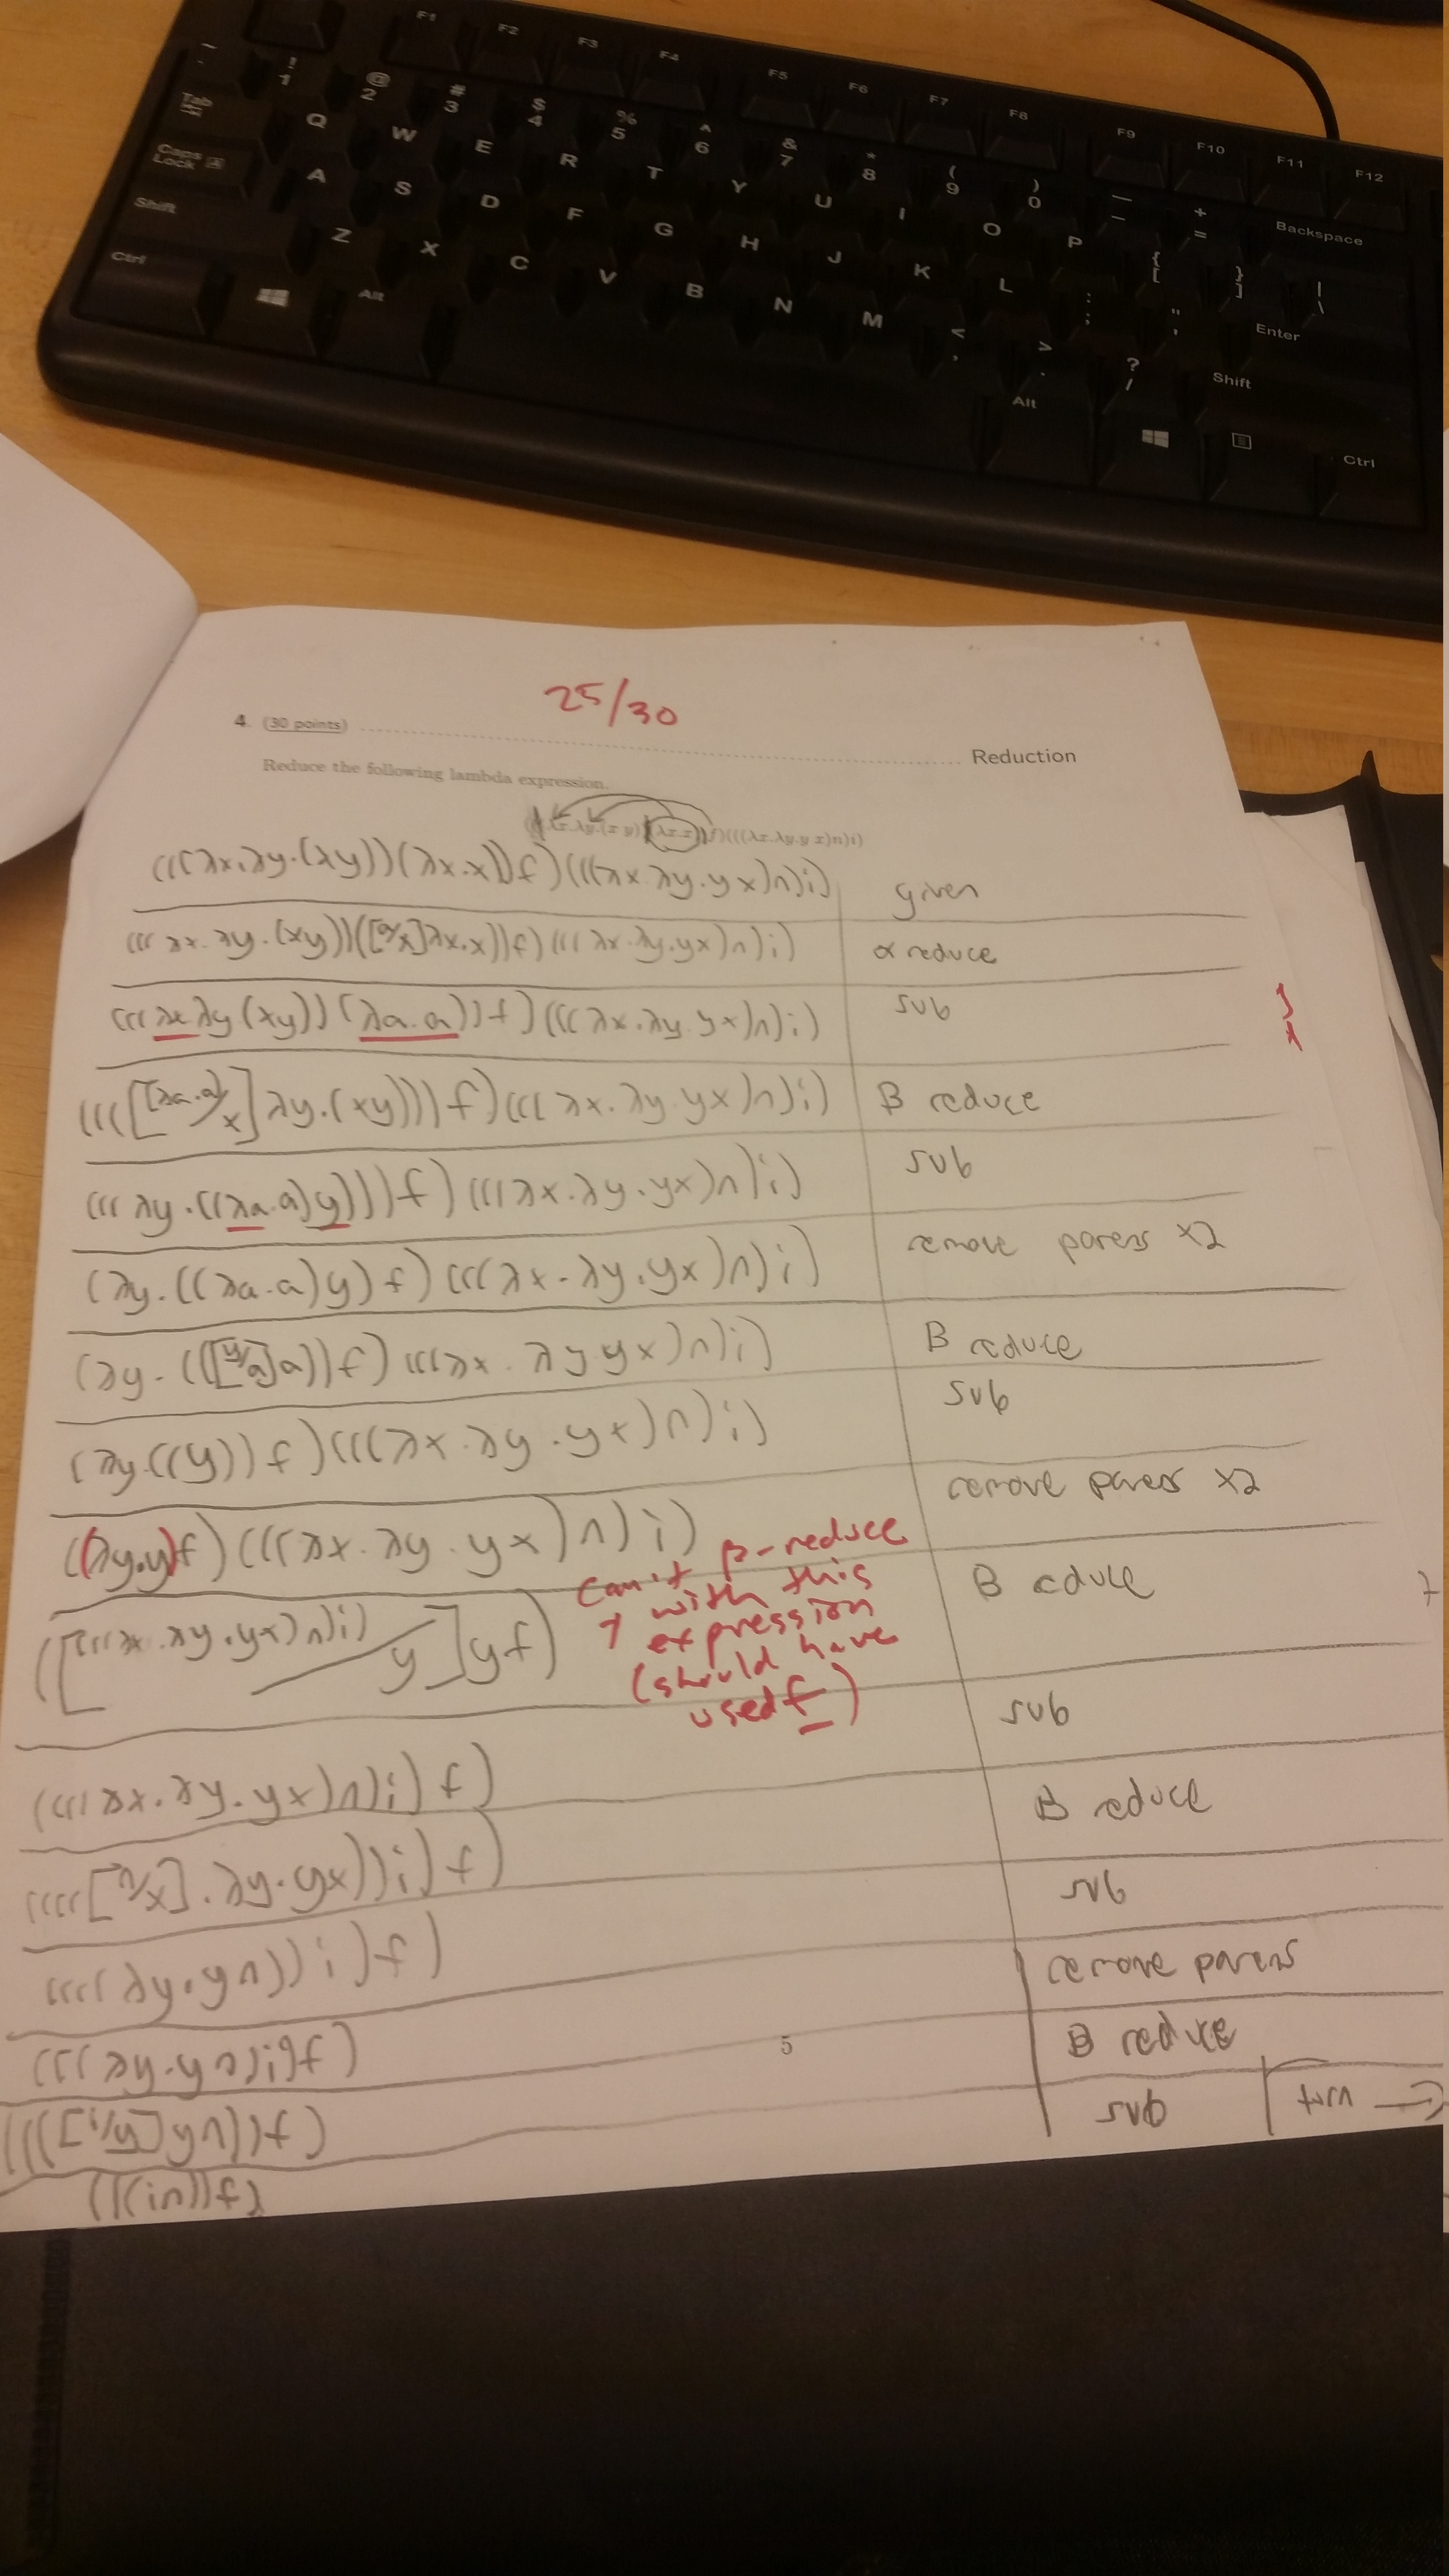
\includegraphics[width=0.33\textwidth]{images/m3.jpg}
    \end{center}

    I removed parenthesis that were essential in determining what could be evaluated, and thus evaluated the rest of the expression slightly wrong, arriving at the answer `inf`.
  
  new answer:

  \vspace{\baselineskip}

 
    $$
  \begin{aligned}
    (((\lambda x.\lambda y.(xy))(\lambda x.x))f)(((\lambda x. \lambda y. yx)n)i)\qquad &|\qquad given\\
    (((\lambda x.\lambda y.(xy))([a/x]\lambda x.x))f)(((\lambda x. \lambda y. yx)n)i)\qquad &|\qquad \alpha\: reduce\\ 
    (((\lambda x.\lambda y.(xy))(\lambda a.a))f)(((\lambda x. \lambda y. yx)n)i)\qquad &|\qquad  sub\\
    ((([(\lambda a.a)/x]\lambda y.(xy)))f)(((\lambda x. \lambda y. yx)n)i)\qquad &|\qquad \beta\: reduce\\
    (((\lambda y.((\lambda a.a)y)))f)(((\lambda x. \lambda y. yx)n)i)\qquad &|\qquad sub\\
    (((\lambda y.(([y/a]a))))f)(((\lambda x. \lambda y. yx)n)i)\qquad &|\qquad \beta\: reduce \\
    (((\lambda y.((y))))f)(((\lambda x. \lambda y. yx)n)i)\qquad &|\qquad sub \\
    ((\lambda y.y)f)(((\lambda x. \lambda y. yx)n)i)\qquad &|\qquad remove\: parens(*3) \\
    (([f/y]y))(((\lambda x. \lambda y. yx)n)i)\qquad &|\qquad \beta\: reduce\\
    ((f))(((\lambda x. \lambda y. yx)n)i)\qquad &|\qquad sub\\
    f(((\lambda x. \lambda y. yx)n)i)\qquad &|\qquad remove\: parens(*2)\\
    f((([n/x]. \lambda y. yx))i)\qquad &|\qquad \beta\: reduce\\
    f(((\lambda y. yn))i)\qquad &|\qquad sub\\
    f((([i/y]. yn)))\qquad &|\qquad \beta\: reduce\\
    f(((in)))\qquad &|\qquad sub\\
    fin\qquad &|\qquad  remove\: parens(*3)\\
  \end{aligned}
  $$


  
\end{enumerate}

% DO NOT DELETE ANYTHING BELOW THIS LINE
\end{document}
